\documentclass[a4]{article}
\usepackage{gnuplottex}
\usepackage{csvsimple}
\usepackage{subcaption}
\usepackage{amsmath}
\usepackage{indentfirst}
\usepackage{float}


\title{COMP26120 Lab 5 Report}
\author{XINYU LI}
\begin{document}
\maketitle

\newpage
\section{What makes a problem hard for Dynamic Programming?}

\subsection{Hypothesis}

The weight capacity of the knapsack might make the problem harder for a dynamic programming solution. The increase of knapsack capacity will cause the running time of dynamic programming algorithm to become longer and vice versa.

\subsection{Design}

Throughout the experiment, the knapsack capacity size ranged from 100 to 15000 with an interval of 100. To create the input files, I ran the kp\_generate.py file through the os.system statement in Jupyter Notebook and created 149 text documents containing the input. \\

I created three experiments with different amount of items and caps on profit and weight per item, but kept these two variables constant in single experiments. \\

In experiment 1, the amount of item is 50000, the cap on profit and weight per item is 1000. In experiment 2, the amount of item is 20000, the cap on profit and weight per item is 2000. In experiment 3, the amount of item is 10000, the cap on profit and weight per item is 3000. \\

In the for loop, I use the time.time() statement to record the time at the start and end of each loop and use the difference as the time to run a test. The pack volume and its corresponding run time are put into a dataframe and exported as a csv file. Finally a scatter plot is used to represent the relationship between the two. 

\subsection{Results}

\noindent The results show in the end part of python/experiment1/experiment1.ipynb, python/experiment2/experiment2.ipynb, python/experiment3/experiment3.ipynb.

\begin{figure}[H]
    \begin{minipage}{0.32\textwidth}        
    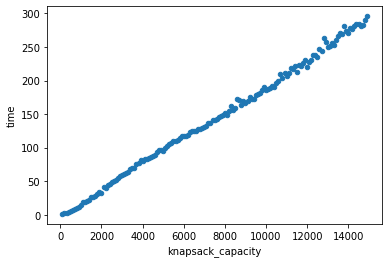
\includegraphics[width=0.95\textwidth]{python/experiment1/output1.png}
    \caption{Capacity-Time}
    \end{minipage}
    \begin{minipage}{0.32\textwidth}        
    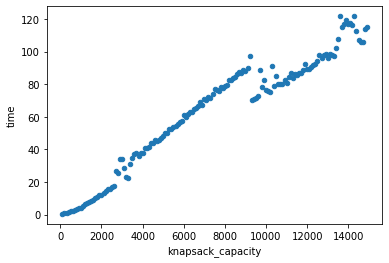
\includegraphics[width=0.95\textwidth]{python/experiment2/output2.png}
    \caption{Capacity-Time}
    \end{minipage}
    \begin{minipage}{0.32\textwidth}        
    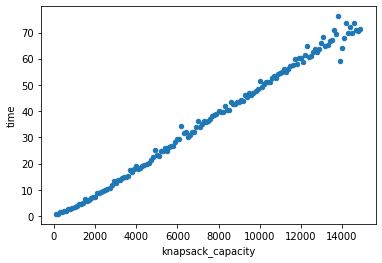
\includegraphics[width=0.95\textwidth]{python/experiment3/output3.png}
    \caption{Capacity-Time}
    \end{minipage}
\end{figure}

\newpage
\subsection{Discussion}

According to my experiment results, there is a positive correlation between the knapsack capacity and the running time of the dynamic programming algorithm. This suggests that increasing the knapsack capacity can make the dynamic programming algorithm more difficult to solve. This is because with an increased capacity, there may be more options to consider, which could lead to longer processing times for the dynamic programming algorithm. Conversely, when the knapsack capacity is decreased, there are fewer options to consider, which results in a corresponding decrease in the algorithm's running time. \\

It is worth noting that in Experiments 1 and 2, I used more items than the capacity of the knapsack, at which point the backpack problem existed. However, in Experiment 3, the number of items I used was 10,000 and the capacity of the knapsack was 15,000, so the knapsack capacity was greater than the number of items and the knapsack problem did not exist, but the program still ran and still showed a positive proportional relationship, which means that my algorithm could be further optimised.

\subsection{Data Statement}

\noindent All data and scripts I used or generated can be found in lab5/python/experiment1, lab5/python/experiment2 and lab5/python/experiment3 \\

\noindent experiment1/experiment1.ipynb

\noindent experiment1/test\_result\_1.csv\\

\noindent experiment2/experiment2.ipynb

\noindent experiment2/test\_result\_2.csv\\

\noindent experiment3/experiment3.ipynb

\noindent experiment3/test\_result\_3.csv

\appendix

%% Any raw data or code scripts you want to present should be included as appendices.
\end{document}
